\vspace{\baselineskip}
Après l’application de l’algorithme de \textit{clustering} sur chacun des
corpus. On a comme résultat un dendrogramme pour chacunes des caractéristique :

\begin{figure}[htbp]
    \centering
    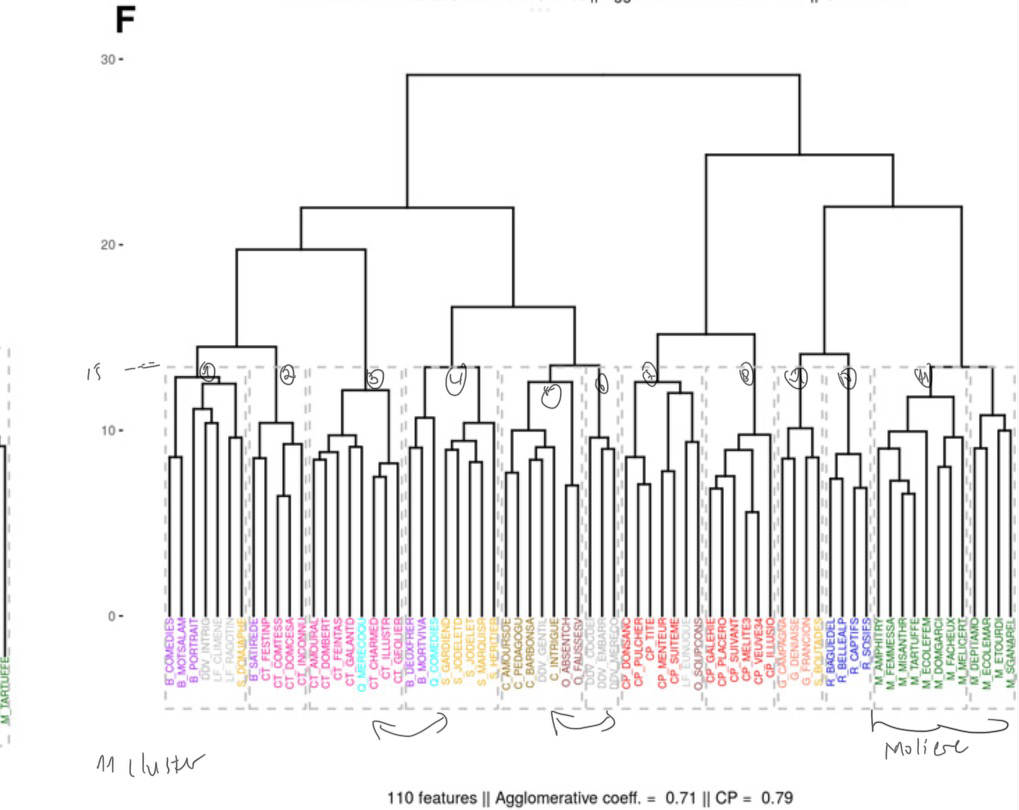
\includegraphics[width=10cm]{Ressources/IMG_0552.png}
    \caption{Dendrogramme mots fonctionels}
    \label{fig:images}
  \end{figure}
  \vspace{\baselineskip}

  \begin{figure}[htbp]
    \centering
    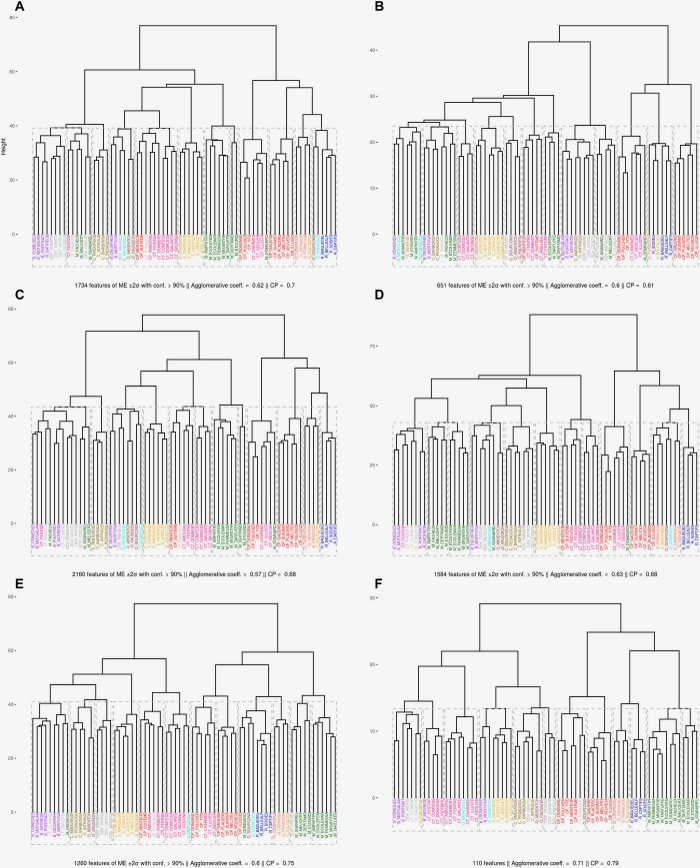
\includegraphics[width=10cm]{Ressources/Fig. 1 JPEG-1.png}
    \caption{Dendrogramme de toutes les caractéristiques}
    \label{fig:images}
  \end{figure}
  

\begin{figure}[htbp]
    De cette interprétation, il en ressort une réfutation des hypothèses énoncées
précédemment. En effet, comme indiqué sur la photo, on peut observer une
distinction claire du cluster attribué à Molière par rapport aux autres auteurs.
Cette distinction remet en question les hypothèses selon lesquelles Molière
aurait pu emprunter les intrigues ou les vers d'autres auteurs, ou encore que
son nom aurait été utilisé comme une simple marque de promotion dissimulant les
véritables auteurs. Les résultats obtenus grâce à l'analyse statistique et à
l'algorithme de clusterisation hiérarchique confirment ainsi l'unicité du style
d'écriture de Molière.
\end{figure}